\section{Prospetto economico}
Vengono mostrati i prospetti economici per ciascun periodo di progetto, divisi per ruolo. I periodi di \AR{} e \AD{} non sono a carico del Committente.

\subsection{\AR}
Nel periodo di \AR{} le ore sono suddivise nel modo seguente:

I seguenti grafici mostrano visivamente come influiranno i ruoli per ore e costi nel periodo di \AR.
\begin{figure}[H]
	\centering
	\includegraphics[width=14cm]{img_peconomico/AA_OR.png}
	\caption{Ore per ruoli, periodo di \AR}
\end{figure}
\begin{figure}[H]
	\centering
	\includegraphics[width=14cm]{img_peconomico/AA_CR.png}
	\caption{Costi per ruolo, periodo di \AR}
\end{figure}

\subsection{\AD}
Nel periodo di \AD{} le ore sono suddivise nel modo seguente:

I seguenti grafici mostrano visivamente come influiranno i ruoli per ore e costi nel periodo di \AD.
\begin{figure}[H]
	\centering
	\includegraphics[width=14cm]{img_peconomico/AD_OR.png}
	\caption{Ore per ruoli, periodo di \AD}
\end{figure}
\begin{figure}[H]
	\centering
	\includegraphics[width=14cm]{img_peconomico/AD_CR.png}
	\caption{Costi per ruolo, periodo di \AD}
\end{figure}

\subsection{\PA}
Nel periodo di \PA{} le ore sono suddivise nel modo seguente:

I seguenti grafici mostrano visivamente come influiranno i ruoli per ore e costi nel periodo di \PA.
\begin{figure}[H]
	\centering
	\includegraphics[width=14cm]{img_peconomico/PA_OR.png}
	\caption{Ore per ruoli, periodo di \PA}
\end{figure}
\begin{figure}[H]
	\centering
	\includegraphics[width=14cm]{img_peconomico/PA_CR.png}
	\caption{Costi per ruolo, periodo di \PA}
\end{figure}

\subsection{\PD}
Nel periodo di \PD{} le ore sono suddivise nel modo seguente:

I seguenti grafici mostrano visivamente come influiranno i ruoli per ore e costi nel periodo di \PD{}.
\begin{figure}[H]
	\centering
	\includegraphics[width=14cm]{img_peconomico/PD_OR.png}
	\caption{Ore per ruoli, periodo di \PD}
\end{figure}
\begin{figure}[H]
	\centering
	\includegraphics[width=14cm]{img_peconomico/PD_CR.png}
	\caption{Costi per ruolo, periodo di \PD}
\end{figure}

\subsection{\Cod}
Nel periodo di \Cod{} le ore sono suddivise nel modo seguente:

I seguenti grafici mostrano visivamente come influiranno i ruoli per ore e costi nel periodo di \Cod.
\begin{figure}[H]
	\centering
	\includegraphics[width=14cm]{img_peconomico/C_OR.png}
	\caption{Ore per ruoli, periodo di \Cod}
\end{figure}
\begin{figure}[H]
	\centering
	\includegraphics[width=14cm]{img_peconomico/C_CR.png}
	\caption{Costi per ruolo, periodo di \Cod}
\end{figure}

\subsection{\VV}
Nel periodo di \VV{} le ore sono suddivise nel modo seguente:

I seguenti grafici mostrano visivamente come influiranno i ruoli per ore e costi nel periodo di \VV{}.
\begin{figure}[H]
	\centering
	\includegraphics[width=14cm]{img_peconomico/VV_OR.png}
	\caption{Ore per ruolo, periodo di \VV}
\end{figure}
\begin{figure}[H]
	\centering
	\includegraphics[width=14cm]{img_peconomico/VV_CR.png}
	\caption{Costi per ruolo, periodo di \VV}
\end{figure}

\subsection{Totale}
\subsubsection{Ore totali con investimento}
Le ore complessive previste per ogni ruolo sono riportate nella tabella sottostante.
I seguenti grafici mostrano visivamente come influiranno i ruoli per ore e costi nel progetto.
\begin{figure}[H]
	\centering
	\includegraphics[width=14cm]{img_peconomico/T_OR_C.png}
	\caption{Ore totali per ruolo}
\end{figure}
\begin{figure}[H]
	\centering
	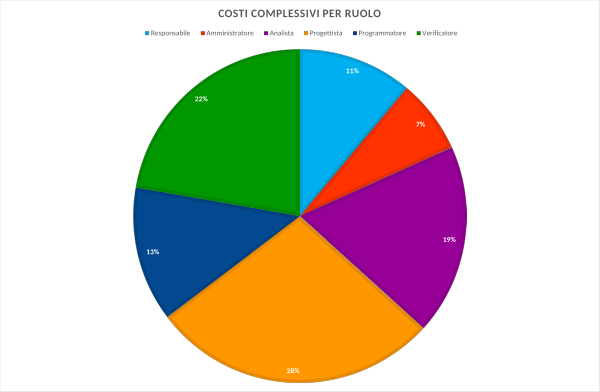
\includegraphics[width=14cm]{img_peconomico/T_CR_C.png}
	\caption{Costi totali per ruolo}
\end{figure}

\subsubsection{Ore totali senza investimento}
Le ore complessive rendicontate per ogni ruolo, cioè quelle senza investimento iniziale, sono riportate nella tabella sottostante.
I seguenti grafici mostrano visivamente come influiranno i ruoli per ore e costi nel progetto.
\begin{figure}[H]
	\centering
	\includegraphics[width=14cm]{img_peconomico/T_OR_R.png}
	\caption{Ore totali senza investimento per ruolo}
\end{figure}
\begin{figure}[H]
	\centering
	\includegraphics[width=14cm]{img_peconomico/T_CR_R.png}
	\caption{Costi totali senza investimento per ruolo}
\end{figure}





